\documentclass[10pt,leqno]{amsart}
\usepackage{graphicx}
\baselineskip=16pt

\usepackage{indentfirst,csquotes}

\topmargin= .5cm
\textheight= 22.5cm
\textwidth= 32cc
\baselineskip=16pt

\evensidemargin= .9cm
\oddsidemargin= .9cm

\usepackage{amssymb,amsthm,amsmath}
\usepackage{xcolor,paralist,hyperref,titlesec,fancyhdr,etoolbox}
\newtheorem{theorem}{Theorem}[]
\newtheorem{definition}[theorem]{Definition}
\newtheorem{example}[theorem]{Example}
\newtheorem{lemma}[theorem]{Lemma}
\newtheorem{proposition}[theorem]{Proposition}
\newtheorem{corollary}[theorem]{Corollary}
\newtheorem{conjecture}[theorem]{Conjecture}

\titleformat{\section}[display]{\normalfont\huge\bfseries\centering}{\centering\chaptertitlename\thechapter}{10pt}{\Large}
\titlespacing*{\section}{0pt}{0ex}{0ex}

\hypersetup{ colorlinks=true, linkcolor=black, filecolor=black, urlcolor=black }
\def\proof{\noindent {\it Proof. $\, $}}
\def\endproof{\hfill $\Box$ \vskip 5 pt }

% --- Additions to the proposal template (report only) -----------------------
\usepackage{booktabs}
% The template's \titleformat breaks \section in amsart (\chaptertitlename is
% undefined), so headings follow the proposal's bold run-in style.
\newcommand{\heading}[1]{\medskip\noindent\textbf{#1}\par}
% All numbers below come from src/report_assets.py (do not type them by hand).
% Generated by src/report_assets.py -- do not edit by hand.
\newcommand{\DataNiftyDays}{4{,}740}
\newcommand{\DataVixMonths}{196}
\newcommand{\DataVixVerified}{4{,}032}
\newcommand{\DataYahooMissing}{47}
\newcommand{\FoAtmViolPct}{0.28}
\newcommand{\FoDays}{4{,}031}
\newcommand{\FoExpiries}{194}
\newcommand{\FoIVcorr}{0.96}
\newcommand{\FoParityBand}{28}
\newcommand{\FoParityPairs}{136{,}118}
\newcommand{\IvrOptAbove}{73}
\newcommand{\IvrOptIvMean}{15.7}
\newcommand{\IvrOptRvMean}{14.5}
\newcommand{\IvrOptVarRatioCovid}{0.68}
\newcommand{\IvrOptVarRatioEx}{1.20}
\newcommand{\IvrVixAbove}{79}
\newcommand{\IvrVixMean}{17.1}
\newcommand{\IvrVixRvMean}{14.7}
\newcommand{\IvrVixVarRatioCovid}{0.73}
\newcommand{\IvrVixVarRatioEx}{1.36}
\newcommand{\OptDailyJ}{57.7}
\newcommand{\OptMeanPnl}{18}
\newcommand{\OptOptions}{1{,}898}
\newcommand{\OptOwnVsVix}{\ensuremath{-4.3}\%}
\newcommand{\OptOwnVsVixz}{\ensuremath{-1.5}}
\newcommand{\OptPremium}{179}
\newcommand{\ParAlpha}{0.527}
\newcommand{\ParHurst}{0.027}
\newcommand{\ParVolZero}{8.9}
\newcommand{\ParVzero}{0.0079}
\newcommand{\RegMSRatio}{1.74}
\newcommand{\RegMSRatioLo}{1.40}
\newcommand{\RegMSsigCalm}{0.71}
\newcommand{\RegMSsigStress}{1.23}
\newcommand{\RegRvQ}{17.4}
\newcommand{\RegVixQ}{20.16}
\newcommand{\RegVixQlo}{17.88}
\newcommand{\RepBS}{0.732}
\newcommand{\RepBSStored}{0.726}
\newcommand{\RepGKW}{0.828}
\newcommand{\RepGKWStored}{0.824}
\newcommand{\SimFlatSteps}{62}
\newcommand{\SimGKWvsBSzMax}{\ensuremath{-6.2}}
\newcommand{\SimGKWvsBSzMin}{\ensuremath{-5.1}}
\newcommand{\SimLowGainMax}{31\%}
\newcommand{\SimLowGainMin}{6\%}
\newcommand{\SimLowHoldoutAgree}{15/16}
\newcommand{\SimOptBSChange}{\ensuremath{-5.9}\%}
\newcommand{\SimOptBSz}{\ensuremath{-1.7}}
\newcommand{\SimOptGKWChange}{\ensuremath{-1.2}\%}
\newcommand{\SimOptGKWz}{\ensuremath{-0.5}}
\newcommand{\SimPaths}{50{,}000}
\newcommand{\SimSteps}{512}
\newcommand{\SynDailyJ}{64.0}
\newcommand{\SynMeanPnl}{30}
\newcommand{\SynOptions}{1{,}914}
\newcommand{\SynPremium}{197}

% -----------------------------------------------------------------------------

\begin{document}
\title{Variance-Optimal Hedging under Rough Volatility and Jumps}
\author{MAC F244: Stochastic Calculus and Applications to Finance \\ Project Report (draft)}
\date{\today}
\maketitle
\vspace{-1.5em}

\let\thefootnote\relax
\footnotetext{MSC2020: Primary 91G20, Secondary 60H30.}

\bigskip

\heading{1. Problem and summary.}
\noindent Black--Scholes theory hedges an option perfectly by holding its delta,
rebalanced continuously and at no cost. Real hedgers trade a few times a day at
most, pay costs, and face markets that switch between calm and stress. We ask
how an option should be hedged under these constraints: how often to rebalance,
whether to trade more in stressed markets, and how much a better hedge ratio is
worth. We answer this in two settings:
\begin{compactitem}
\item \emph{in simulation}, under a realistic model with rough volatility and
clustered crash jumps \cite{BPS24}, using the variance-optimal hedge computed by
the published code of \cite{WW26}, which we reproduce;
\item \emph{on Indian market data}: NIFTY~50, India VIX and traded NIFTY options
(2010--2026). Rules are calibrated on 2010--2018 and evaluated out of sample on
2019--2026.
\end{compactitem}

\heading{2. Hedging: from complete to incomplete markets.}
\noindent Throughout we work under the pricing measure $\mathbb{Q}$ with zero
interest rate \cite{Shr04}.

\noindent\emph{(a) Black--Scholes.} Let $dS_t=\sigma S_t\,dW_t$ and let $C(t,S)$ be
the call price, which solves $C_t+\frac12\sigma^2S^2C_{SS}=0$. By It\^o's formula
the $dt$-terms of $dC$ cancel, so $dC=C_S\,dS$. Holding $\Delta=C_S$ shares
therefore replicates the call exactly. This is the martingale representation
theorem at work in a complete market.

\noindent\emph{(b) Discrete rebalancing.} If $\Delta$ is reset only every $h$ years,
the hedge is frozen while the option's value moves nonlinearly. Let
$\Gamma=C_{SS}$ and let $R_k$ be the return over $[t_k,t_k+h]$. A second-order
expansion with $C_t=-\frac12\sigma^2S^2\Gamma$ gives the short-call hedging error
over one interval:
\[
\varepsilon_k\approx\tfrac12\Gamma_kS_k^2\big(\sigma^2h-R_k^2\big),\qquad
\mathrm{Var}(\varepsilon_k)\approx\tfrac12\Gamma_k^2S_k^4\sigma^4h^2 .
\]
Summed over the $T/h$ intervals, the extra variance is of order $h$: it roughly
doubles when the interval doubles.

\noindent\emph{(c) Gamma P\&L.} If the delta is computed at an implied volatility
$\sigma_i$ while the stock moves with realised volatility $\sigma_r$, then
$\mathbb{E}[R_k^2]\approx\sigma_r^2h$. The delta-hedged seller therefore earns on
average
\[
\tfrac12\,\Gamma S^2\big(\sigma_i^2-\sigma_r^2\big)\,dt ,
\]
which is positive when implied volatility exceeds the volatility that follows.

\noindent\emph{(d) Incomplete markets and the minimum-variance hedge.} With
stochastic volatility or jumps there are more sources of risk than traded
assets, so no stock position replicates the call. The best one can do is to
minimise $\mathbb{E}^{\mathbb{Q}}[(Y-x-\int_0^T\vartheta_t\,dS_t)^2]$ for the payoff
$Y=(S_T-K)^+$. Write $M_t=\mathbb{E}^{\mathbb{Q}}[Y\mid\mathcal F_t]$ (the option
price) and decompose $Y=\mathbb{E}^{\mathbb{Q}}[Y]+\int_0^T\vartheta^*_t\,dS_t+L_T$,
with the residual $L$ uncorrelated with $S$ (the Galtchouk--Kunita--Watanabe
decomposition \cite{FS86}). Then, for any $(x,\vartheta)$,
\[
\mathbb{E}\Big[\Big(Y-x-\int_0^T\vartheta\,dS\Big)^2\Big]
=(\mathbb{E}[Y]-x)^2+\mathbb{E}\int_0^T(\vartheta^*-\vartheta)^2d\langle S\rangle+\mathbb{E}[L_T^2],
\]
so the optimum is $x=\mathbb{E}^{\mathbb{Q}}[Y]$ (the price) and
\[
\vartheta^*_t=\frac{d\langle M,S\rangle_t}{d\langle S\rangle_t},
\]
a regression of option moves on stock moves. $\mathbb{E}[L_T^2]$ is the risk no
stock position can remove. \emph{Example (Heston):} for $dS=\sqrt{v}\,S\,dW$ and
$dv=\kappa_v(\theta-v)\,dt+\xi\sqrt{v}\,dB$ with $d\langle W,B\rangle=\rho\,dt$,
write $M_t=C(t,S_t,v_t)$. Two-variable It\^o gives
$d\langle M,S\rangle=(C_S\,vS^2+C_v\,\rho\xi vS)\,dt$ and $d\langle S\rangle=vS^2\,dt$, so
\[
\vartheta^*=C_S+\frac{\rho\,\xi\,C_v}{S}.
\]
With $\rho<0$ (volatility rises when prices fall) and $C_v>0$, the
variance-optimal hedge holds fewer shares than the delta.

\noindent\emph{(e) The simulation model.} For simulation we use the rough
Hawkes--Heston model \cite{BPS24}. It is a Heston-type model whose variance has
long memory (it depends on all past shocks through a power-law kernel, giving
``rough'' paths) and whose price has crash jumps that become more likely after
a jump. Wang and Wang \cite{WW26} derive $\vartheta^*$ for this model. It has
the covariance structure of (d) plus a jump term, and it is computed with
Fourier and Riccati--Volterra methods. We use the authors' published
implementation \cite{WWcode}.

\noindent\emph{(f) Discrete trading with costs.} We trade a target hedge
($\vartheta^*$ or a delta) only at dates $t_0<\dots<t_{N-1}$, holding $\varphi_k$
shares on $(t_k,t_{k+1}]$. With a proportional cost $\kappa$ per unit of traded
notional, the short-call P\&L is
\[
e = x + \sum_{k=0}^{N-1}\varphi_k(S_{k+1}-S_k)
 - \kappa\sum_{k=0}^{N-1}S_k|\varphi_k-\varphi_{k-1}| - \kappa S_N|\varphi_{N-1}| - Y,
 \qquad \varphi_{-1}=0 .
\]
A rebalancing rule chooses when $\varphi$ is reset to its target. The rules are:
\emph{fixed} (every $m$ steps); \emph{regime-aware} (every $m_{\rm stress}$ steps in
stress, $m_{\rm calm}$ otherwise); and a \emph{no-trade band} (trade when the target
moves more than $h$ shares). Every rule uses only information up to $t_k$.

\heading{3. Replication.}
\noindent Running the official code \cite{WWcode} (\SimPaths{} paths, $T=0.25$,
ATM call) reproduces its results (Table~\ref{tab:rep}). Measured as the
reduction in hedging-error variance against not hedging, it gives \RepGKW{} for
the variance-optimal (GKW) hedge and \RepBS{} for the Black--Scholes delta. These
numbers are official-code output rather than results printed in \cite{WW26}. The
small differences from the stored values come from a different random stream
and lie within one standard error. The paper's own convergence tables also
reproduce.

\begin{table}[h]
\centering\small
\begin{tabular}{lcc}
\toprule
Hedge & Official output & Our rerun \\
\midrule
Variance-optimal (GKW) hedge & 0.824 & 0.828 \\
Black--Scholes delta (implied vol) & 0.726 & 0.732 \\
\bottomrule
\end{tabular}

\caption{Variance reduction vs.\ no hedge, \SimPaths{} paths, \SimSteps{} steps.}
\label{tab:rep}
\end{table}

\heading{4. Discrete rebalancing with costs (simulation).}
\noindent We reuse the official market simulation and hedge, and change only the
trading dates and the costs. All rules are evaluated on the same paths, so
comparisons use paired standard errors. With fewer rebalancing dates the
variance reduction falls for both hedges, as Section~2(b) predicts. The GKW
advantage over the BS delta \emph{grows} (Table~\ref{tab:freq}): the better hedge
ratio matters more when the position is held longer. With costs, GKW beats BS at every cost
level ($z$ between \SimGKWvsBSzMin{} and \SimGKWvsBSzMax{}). To compare rules
fairly, each band or regime rule is set against a randomised mixture of the two
neighbouring fixed rules with the same expected turnover, and hence the same
expected cost. At low turnover these rules reduce the mean squared error by
\SimLowGainMin{}--\SimLowGainMax{} at $\kappa=10$\,bp, and the sign agrees on an
independent seed in \SimLowHoldoutAgree{} cases. At the cost-optimal point,
however, frequent trading is optimal and the rules nearly coincide. Against the
best fixed rule, the best smart rule changes the mean squared error by only
\SimOptGKWChange{} ($z=\SimOptGKWz$) for GKW and \SimOptBSChange{} ($z=\SimOptBSz$)
for BS.

\begin{table}[h]
\centering\small
\begin{tabular}{rcc}
\toprule
Rebalancing dates & GKW hedge & BS delta \\
\midrule
512 & 0.828 (0.012) & 0.732 (0.026) \\
64 & 0.806 (0.013) & 0.670 (0.031) \\
16 & 0.738 (0.016) & 0.541 (0.033) \\
4 & 0.583 (0.021) & 0.333 (0.036) \\
1 & 0.374 (0.019) & 0.108 (0.036) \\
\bottomrule
\end{tabular}

\caption{Variance reduction (standard error) against the number of rebalancing dates, $\kappa=0$.}
\label{tab:freq}
\end{table}

\begin{figure}[h]
\centering
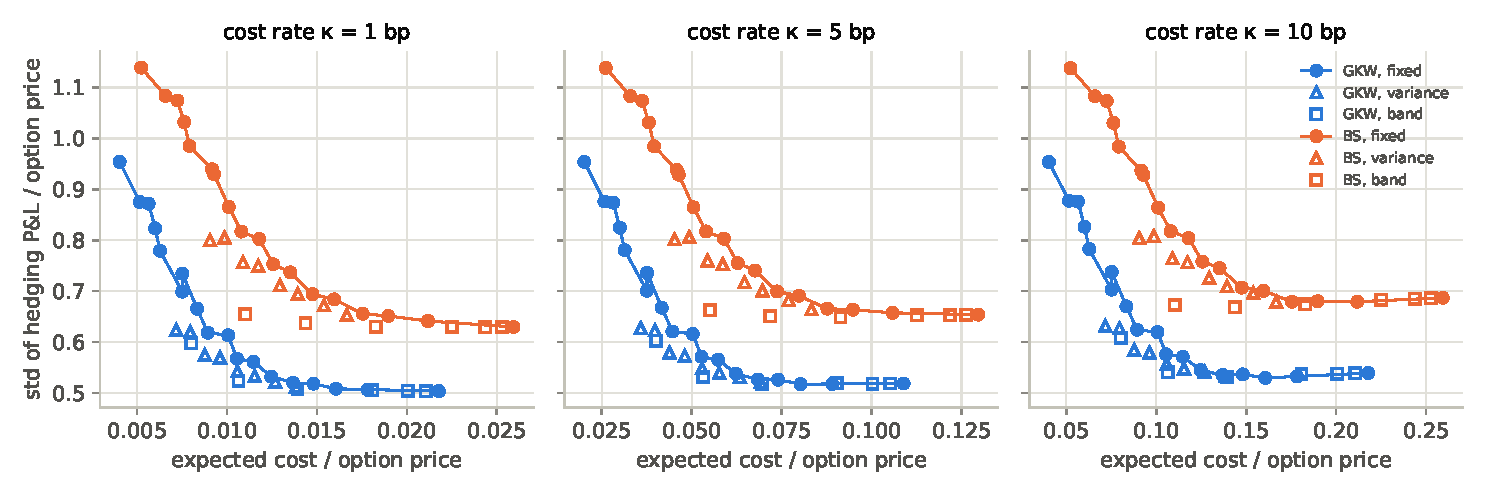
\includegraphics[width=\textwidth]{figures/sim_frontier.pdf}
\caption{Simulation: standard deviation of the P\&L against expected cost (both relative to the option price) for each rule.}
\label{fig:simfrontier}
\end{figure}

\heading{5. Data and regimes.}
\noindent We use the official NIFTY~50 closes (NSE Indices, \DataNiftyDays{} days;
Yahoo Finance agrees on common days but misses \DataYahooMissing{}) and India VIX
from Yahoo, patched and verified against NSE (\DataVixVerified{} days from July
2010, all \DataVixMonths{} months checked) \cite{NSEidx,NSEvix}. Regimes are
estimated on 2010--2018 only. The main label is India VIX above \RegVixQ{}, with
hysteresis down to \RegVixQlo{} so that the label does not flicker. The second
label is 21-day realised volatility above \RegRvQ\%. Each label at $t$ uses data up
to $t$ only, which we check by truncating the data at $t$. Out of sample, stress
labels are followed by 1.7--2.0 times higher realised volatility
(Table~\ref{tab:reg}, Figure~\ref{fig:reg}). A third, statistical label (a
two-state Markov-switching model of returns \cite{Ham89}) is used only as a
robustness check and gives the same picture (ratio \RegMSRatio, lower 95\% bound
\RegMSRatioLo).

\begin{table}[h]
\centering\small
\begin{tabular}{lcc}
\toprule
Variant & VIX (hysteresis) & 21-day realised vol \\
\midrule
Main (train to 2018) & 1.94 [1.58, 2.44] & 1.79 [1.37, 2.41] \\
Train to 2017 & 1.94 [1.57, 2.46] & 1.80 [1.37, 2.38] \\
Train to 2019 & 2.01 [1.65, 2.54] & 1.85 [1.40, 2.47] \\
Start 2008 (unverified VIX) & 2.25 [1.52, 3.35] & 1.86 [1.32, 2.64] \\
\bottomrule
\end{tabular}

\caption{Test period 2019--2026: realised volatility over the next 5 days after a stress label, divided by that after a calm label [block-bootstrap 95\% CI].}
\label{tab:reg}
\end{table}

\begin{figure}[h]
\centering
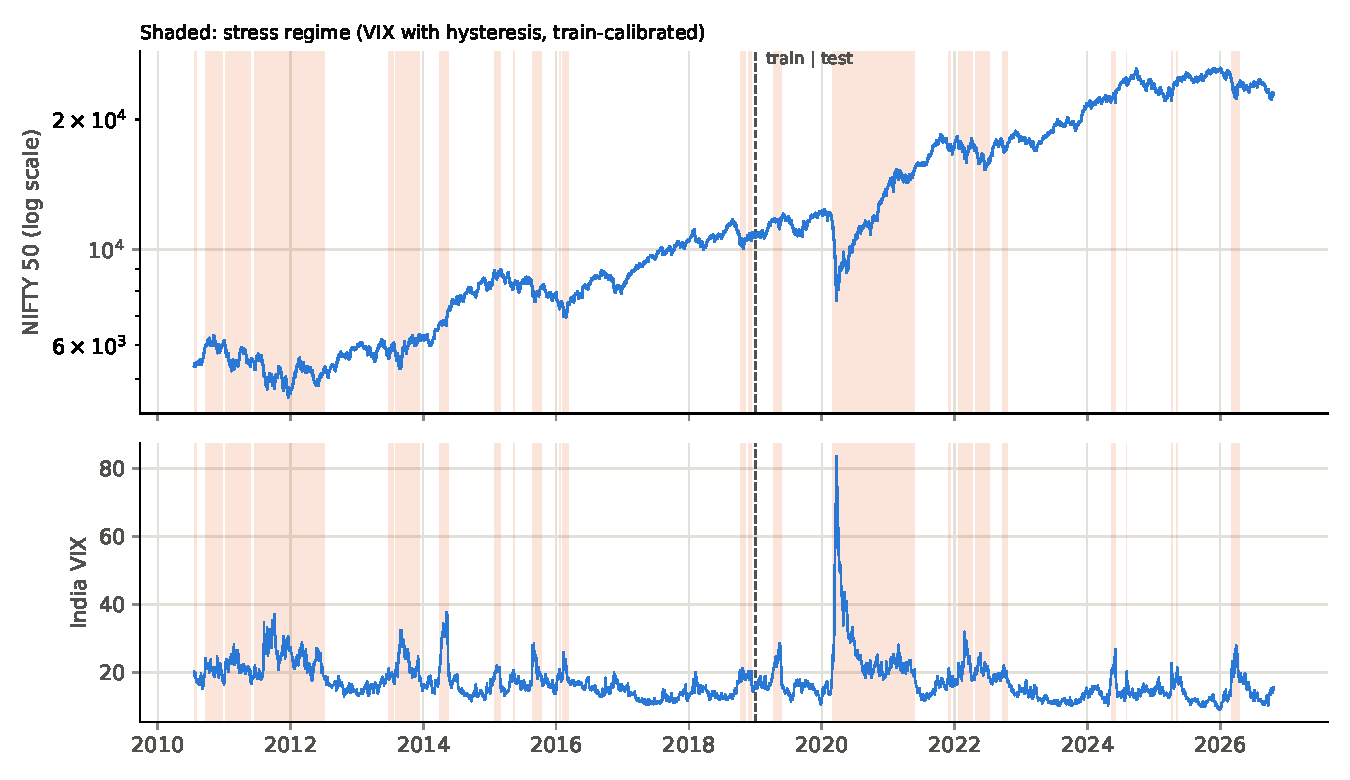
\includegraphics[width=0.9\textwidth]{figures/regimes.pdf}
\caption{NIFTY~50 and India VIX; shaded: stress (VIX with hysteresis).}
\label{fig:reg}
\end{figure}

\heading{6. Backtest on NIFTY with synthetic options.}
\noindent At each close we sell a 21-day ATM call priced at India VIX (Black--Scholes
\cite{Bla76}) and hedge with the delta at the current VIX, giving \SynOptions{} test
options with a mean premium of \SynPremium{}\,bp. The seller's cost-free mean P\&L
is about $+\SynMeanPnl$\,bp. This is the gamma P\&L of Section~2(c), since
implied volatility usually exceeded the volatility that followed. India VIX was
above the next month's realised volatility on \IvrVixAbove\% of test days (mean
\IvrVixMean\% against \IvrVixRvMean\%). In variance terms, implied exceeded
realised by a factor \IvrVixVarRatioEx{} outside the COVID window, while the
crash reversed it (factor \IvrVixVarRatioCovid). Because this mean reflects the
volatility premium rather than hedging quality, we rank rules by
$J=\mathrm{Var}(e)+(\mathbb{E}[\text{cost}])^2$, which equals the simulation
criterion when the premium is fair. Options overlap, so standard
errors use a moving-block bootstrap \cite{Kun89}. Daily rebalancing is the best
rule on the training period at every cost up to 20\,bp, and the regime rule
chosen on train is \emph{worse} on test (Table~\ref{tab:bt}). At equal turnover,
regime-aware rules appear better on the full test period, but this comes from
the 2020 COVID crash: excluding it, or using 63-day options, the advantage
disappears. Rules driven by inverted labels are worse than those driven by the
real labels, so trading less in stress clearly hurts. Trading more in stress,
however, does not reliably beat a fixed schedule.

\begin{table}[h]
\centering\small
\begin{tabular}{lccccc}
\toprule
 & \multicolumn{2}{c}{Picked on train vs daily} & \multicolumn{3}{c}{Equal turnover, 5\,bp} \\
\cmidrule(lr){2-3}\cmidrule(lr){4-6}
Variant & 5\,bp & 20\,bp & beat fixed & med.\ $z$ & beat placebo \\
\midrule
21-day, full test & \ensuremath{+19.5}\% (\ensuremath{2.9}) & \ensuremath{+7.9}\% (\ensuremath{1.6}) & 42/48 & \ensuremath{-1.1} & 46/48 \\
21-day, excl.\ COVID window & \ensuremath{+30.0}\% (\ensuremath{2.7}) & \ensuremath{+9.8}\% (\ensuremath{1.5}) & 20/48 & \ensuremath{0.2} & 34/48 \\
63-day options & \ensuremath{+8.1}\% (\ensuremath{3.3}) & \ensuremath{+2.7}\% (\ensuremath{1.0}) & 19/48 & \ensuremath{0.3} & 35/48 \\
\bottomrule
\end{tabular}

\caption{Synthetic-option backtest, test period. Left: change in $J$ of the
regime rule picked on train vs.\ daily rebalancing ($z$). Right: regime rules
(4 labels $\times$ 12 settings) vs.\ fixed rules at equal turnover, and how
often they beat the inverted-label placebo.}
\label{tab:bt}
\end{table}

\heading{7. Backtest with traded NIFTY options.}
\noindent We repeat Section~6 with traded prices from the NSE F\&O bhavcopies
\cite{NSEfo} (\FoDays{} trading days, 2010--2026). The data pass basic checks:
\begin{compactitem}
\item at all \FoExpiries{} monthly expiries the expiring future settles exactly at the NIFTY close;
\item near-ATM put--call parity holds within $\pm\FoParityBand$\,bp (1st--99th percentile, \FoParityPairs{} pairs);
\item only \FoAtmViolPct\% of traded near-ATM calls violate no-arbitrage bounds;
\item ATM implied volatility has correlation \FoIVcorr{} with India VIX.
\end{compactitem}
Expiries moved for holidays are detected from the data. At each close we sell the
monthly call closest to 21 trading days from expiry, at the strike nearest the
futures price and at its traded close. We hedge with the same-expiry future at
the Black--76 delta \cite{Bla76}, using the option's own implied volatility; both
contracts settle on the index at expiry. This gives \OptOptions{} test options
(mean premium \OptPremium\,bp). Daily hedging reaches a $J$-RMSE of \OptDailyJ\,bp,
against \SynDailyJ\,bp with synthetic options, and the cost-free mean P\&L is
$+\OptMeanPnl$\,bp. Again this is gamma P\&L: the option's implied volatility
exceeded NIFTY's realised volatility over its life for \IvrOptAbove\% of options
(mean \IvrOptIvMean\% against \IvrOptRvMean\%; variance factor \IvrOptVarRatioEx{}
outside the COVID window, \IvrOptVarRatioCovid{} inside it). Using India VIX instead of the option's own implied
volatility in the delta changes $J$ by only \OptOwnVsVix{} ($z=\OptOwnVsVixz$).
The conclusions of Section~6 carry over (Table~\ref{tab:opt},
Figure~\ref{fig:opt}). Daily rebalancing is best on the training period, and
the regime rule picked on train is worse on test. The equal-turnover advantage
of regime-aware rules holds on the full test period but not once the COVID
window is excluded. Real labels again beat the inverted placebo.

\begin{table}[h]
\centering\small
\begin{tabular}{lccccc}
\toprule
 & \multicolumn{2}{c}{Picked on train vs daily} & \multicolumn{3}{c}{Equal turnover, 5\,bp} \\
\cmidrule(lr){2-3}\cmidrule(lr){4-6}
Variant & 5\,bp & 20\,bp & beat fixed & med.\ $z$ & beat placebo \\
\midrule
Own implied vol & \ensuremath{+35.0}\% (\ensuremath{2.1}) & \ensuremath{+15.1}\% (\ensuremath{1.4}) & 48/48 & \ensuremath{-1.0} & 48/48 \\
Own IV, excl.\ COVID window & \ensuremath{+51.8}\% (\ensuremath{2.0}) & \ensuremath{+18.8}\% (\ensuremath{1.3}) & 17/48 & \ensuremath{0.4} & 41/48 \\
India VIX delta & \ensuremath{+33.7}\% (\ensuremath{2.1}) & \ensuremath{+16.3}\% (\ensuremath{1.5}) & 47/48 & \ensuremath{-1.0} & 46/48 \\
\bottomrule
\end{tabular}

\caption{Traded-option backtest, test period (same layout as Table~\ref{tab:bt}).}
\label{tab:opt}
\end{table}

\begin{figure}[h]
\centering
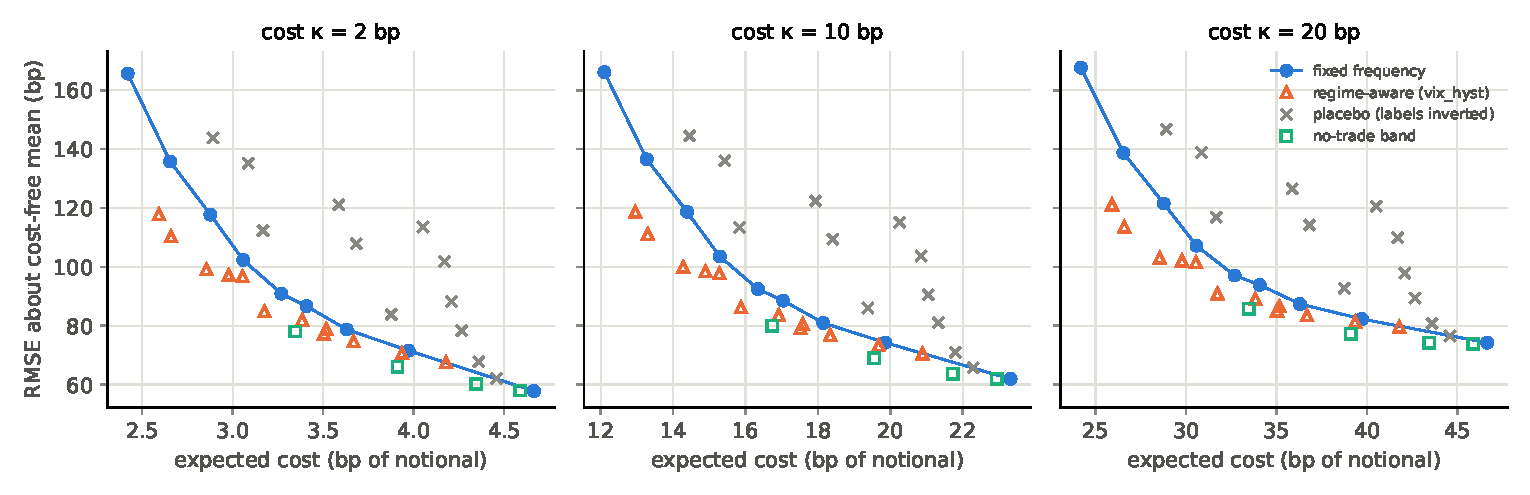
\includegraphics[width=\textwidth]{figures/options_frontier.pdf}
\caption{Traded NIFTY options, test period 2019--2026 (COVID included):
RMSE about the cost-free mean against expected cost, for each rule.}
\label{fig:opt}
\end{figure}

\heading{8. Conclusions and limitations.}
\noindent \emph{Hedge ratio.} Trading the variance-optimal hedge discretely keeps
most of its advantage over the Black--Scholes delta, and the advantage grows as
rebalancing becomes coarser. \emph{Timing.} In simulation and on NIFTY data,
regime-aware rebalancing helps only when turnover must stay low. At realistic
NIFTY costs (up to 20\,bp) daily rebalancing is optimal, and the regime rule
chosen in sample does worse out of sample. The real-data gains at equal turnover
come from a single episode (COVID 2020), so they should not be read as a general
effect. \emph{Profit and loss.} The delta-hedged seller's average gain on NIFTY
is the gamma P\&L of Section~2(c): implied volatility usually exceeded realised
volatility, except in the COVID crash.

\noindent\emph{Limitations.}
\begin{compactitem}
\item The simulation uses one calibration of the model, under $\mathbb{Q}$.
\item The variance-optimal hedge is computed with the authors' published code.
\item The model is not calibrated to NIFTY, so the real-data hedges are
Black--Scholes and Black--76 deltas.
\item Prices are daily closes, which are not perfectly synchronous.
\item Costs are proportional and do not depend on the regime, and margin
financing is ignored.
\item The test period contains essentially one crisis.
\end{compactitem}

\begin{thebibliography}{99}
\bibitem{Shr04} S.~E.~Shreve, \emph{Stochastic Calculus for Finance II:
Continuous-Time Models}, Springer (2004).
\bibitem{WW26} Y.~Wang and X.~Wang, \emph{Variance-optimal hedging in the rough
Hawkes--Heston model}, arXiv:2609.08541 (2026).
\bibitem{WWcode} Y.~Wang and X.~Wang, numerical code,
\url{https://github.com/gagawjbytw/hedging_rough_hawkes_heston} (commit c6a6557, 2026).
\bibitem{BPS24} A.~Bondi, S.~Pulido and S.~Scotti, \emph{The rough Hawkes--Heston
stochastic volatility model}, Math.\ Finance \textbf{34}(4) (2024), 1197--1241.
\bibitem{FS86} H.~F\"ollmer and D.~Sondermann, \emph{Hedging of non-redundant
contingent claims}, in: Contributions to Mathematical Economics, North-Holland (1986).
\bibitem{Bla76} F.~Black, \emph{The pricing of commodity contracts}, J.\ Financial
Economics \textbf{3} (1976), 167--179.
\bibitem{Ham89} J.~D.~Hamilton, \emph{A new approach to the economic analysis of
nonstationary time series and the business cycle}, Econometrica \textbf{57} (1989), 357--384.
\bibitem{Kun89} H.~R.~K\"unsch, \emph{The jackknife and the bootstrap for general
stationary observations}, Ann.\ Statist.\ \textbf{17} (1989), 1217--1241.
\bibitem{NSEidx} NSE Indices Ltd, NIFTY~50 historical data, \url{https://www.niftyindices.com}.
\bibitem{NSEvix} National Stock Exchange of India, India VIX historical data,
\url{https://www.nseindia.com}; Yahoo Finance, \texttt{\^{}INDIAVIX}.
\bibitem{NSEfo} National Stock Exchange of India, F\&O bhavcopy archives,
\url{https://nsearchives.nseindia.com}.
\end{thebibliography}

\bigskip
% Group members. members.tex (with student IDs) is kept out of the public
% repository (see .gitignore); without it, the names-only list is used.
% Public builds define \PublicBuild to force the names-only list.
\ifdefined\PublicBuild
\noindent\textbf{Group members.}\par
\begin{center}
\renewcommand{\arraystretch}{1.25}
\begin{tabular}{|c|p{5cm}|}
\hline
\textbf{No.} & \textbf{Name} \\ \hline
1 & Dhyan Laad \\ \hline
2 & Natasha Nalwaya \\ \hline
3 & Shrirang Bhale \\ \hline
4 & Tanmai Chekuri \\ \hline
5 & Shivam Mahto \\ \hline
\end{tabular}
\end{center}

\else
\IfFileExists{members.tex}{\input{members}}{\noindent\textbf{Group members.}\par
\begin{center}
\renewcommand{\arraystretch}{1.25}
\begin{tabular}{|c|p{5cm}|}
\hline
\textbf{No.} & \textbf{Name} \\ \hline
1 & Dhyan Laad \\ \hline
2 & Natasha Nalwaya \\ \hline
3 & Shrirang Bhale \\ \hline
4 & Tanmai Chekuri \\ \hline
5 & Shivam Mahto \\ \hline
\end{tabular}
\end{center}
}
\fi

\end{document}
